
% !TEX root = ../TGINA template.tex
\section{Experiments and Results}\label{sec:experiments}


Our experiments serve two goals. We first establish that NESS is an effective model for learning under missing node features: it outperforms baselines spanning every category of the problem (Section~\ref{sec:exp-main}), and its advantage widens as features become scarcer (Section~\ref{sec:exp-rate}). We then turn to the study that motivates the paper: not merely whether self-supervision helps, but under which conditions it does and what explains its effectiveness.
We show that its benefit is conditional: only some objectives help (Section~\ref{sec:exp-objectives}), for reasons visible in their mechanism and training dynamics (Section~\ref{sec:exp-why}); the benefit emerges primarily under severe missingness (Section~\ref{sec:exp-missingness-regime}) and on dense rather than sparse binary features (Section~\ref{sec:exp-regime}). Finally, we justify NESS's design choices and establish its transferability and scalability (Sections~\ref{sec:exp-design} and~\ref{sec:exp-scalability}).


\section{Experimental Setup}
\label{sec:setup}

\paragraph{Datasets.} We evaluate on five node-classification benchmarks. Four are small but conventional benchmarks in the graph-missingness literature, citation and co-purchase graphs with sparse binary bag-of-words attributes: Cora, CiteSeer~\cite{yang2016revisiting}, Amazon-Computers (AMAC), and Amazon-Photo (AMAP)~\cite{shchur2018pitfalls}. The fifth, ogbn-arxiv~\cite{hu2020open}, is a large graph with dense, continuous features (169K nodes, 128-dimensional embeddings).
We center our study on ogbn-arxiv as a larger, more realistic benchmark whose dense continuous features and scale expose challenges that small binary graphs do not, making it better suited to studying self-supervision under missingness.
Their statistics are summarized in Table~\ref{tab:datasets}. This spread lets us study behavior across both feature regimes (sparse binary vs.\ dense continuous) and scales. 


\paragraph{Missingness protocol.} 
We simulate attribute-missing conditions by selecting a fraction $\rho$ of nodes uniformly at random and removing their entire feature vector (zero-filled). 
Nodes labels are divided into training, validation, and test splits.
% The feature mask and the label split coincide: the masked nodes are split evenly into validation and test sets, and the remaining feature-observable nodes form the training set
% The classification loss is computed only on observable-node labels, so a node is either feature-observable and used for training or feature-missing and held out for evaluation, and no label or feature information from the evaluated nodes leaks into training.
Message passing operates over the full graph throughout, so missing nodes still receive representations via propagation from their observed neighbors; only their labels and input features are withheld.
We use $\rho=0.4$ for the main comparison against other benchmarks, $0.8$ for the rest of the experiments, and sweep $\rho \in \{0.2,0.4,0.6,0.8,0.9,0.95\}$ for the robustness analysis.



\paragraph{Methods compared.} We compare NESS against baselines spanning every category of the missing-feature landscape. \textbf{NeighAggre} and \textbf{KNN} are non-parametric imputers that fill a missing node from its neighbors or nearest observed nodes~\cite{you2020handling}. \textbf{Feature Propagation} (FP) is a scalable propagation-based imputer that diffuses observed features over the graph~\cite{rossi2022unreasonable}. \textbf{PaGCN} is an imputation-free architecture that aggregates only observed feature entries~\cite{zhang2024incomplete}. \textbf{MATE} is a per-node method that learns a separate embedding for each missing node~\cite{peng2023mate}. \textbf{GraphSAGE} is a standard zero-filled GNN baseline~\cite{hamilton2017inductive}.

We report macro-F1 as the primary metric, along with accuracy on the masked test nodes. All results are averaged over three random seeds.

All learnable methods are trained under an identical budget and protocol: the same number of epochs (800, with early stopping on validation macro-F1, patience of 20 evaluation intervals), the same optimizer (Adam), the same per-dataset learning rate, the same hidden width (128), and the same missingness splits and seeds. Comparisons therefore reflect the methods themselves rather than differences in tuning. The learning rate is $10^{-3}$ for the large and denser graphs (ogbn-arxiv, AMAC), where a higher rate is unstable, and $10^{-2}$ for the remaining small graphs, applied uniformly to every method on a given dataset.

\paragraph{NESS configuration.} Unless otherwise noted, NESS uses a three-layer GraphSAGE encoder of hidden width 128, Feature-Propagation prefill (40 iterations), two independently edge-masked views fused by averaging with a Barlow-Twins contrastive term, and the label-histogram and multi-hop reachability self-supervised objectives. Dropout is 0.3. The loss weights place higher emphasis on the classification term (Section~\ref{sec:experiments} reports the selection). Large graphs are trained with cluster-based batching; small graphs are trained full-batch. Self-supervised targets that depend on global structure are computed once on the full graph and indexed per cluster. The full hyperparameter configuration is discussed in Appendix~\ref{sec:setup-hparams}.

\begin{table}[t]
\centering
\caption{Dataset statistics. ogbn-arxiv is our primary large graph dataset.}
\label{tab:datasets}
\small
\begin{tabular}{@{}lrrrrl@{}}
\toprule
\textbf{Dataset} & \textbf{Nodes} & \textbf{Edges} & \textbf{Features} & \textbf{Classes} & \textbf{Feature type} \\
\midrule
Cora        & 2{,}708     & 5{,}429       & 1{,}433 & 7 & binary BoW \\
CiteSeer    & 3{,}327     & 4{,}732       & 3{,}703 & 6 & binary BoW \\
AMAP        & 7{,}650     & 119{,}081     & 745     & 8 & binary BoW \\
AMAC        & 13{,}752    & 245{,}861     & 767     & 10 & binary BoW \\
ogbn-arxiv  & 169{,}343   & 1{,}166{,}243 & 128     & 40 & dense embedding \\
\bottomrule
\end{tabular}
\end{table}







\subsection{Main Comparison}
\label{sec:exp-main}

We first compare NESS against baselines under random missingness at rate $0.4$. Table~\ref{tab:main} reports test macro-F1 and accuracy on the masked nodes, averaged over three seeds.

On ogbn-arxiv, the large dense-embedding graph that is the primary target of this work, NESS attains the highest performance, reaching $0.454$ macro-F1 compared to $0.439$ for the strongest baseline (FP) and $0.404$ for MATE, and the highest accuracy ($0.676$). NESS also performs favorably on the small binary graphs, achieving the best macro-F1 on CiteSeer ($0.735$) and AMAC ($0.911$) and results within a narrow margin of the best on Cora and AMAP. On these small, sparse benchmarks the strongest methods (FP, PaGCN, MATE) perform comparably and the differences are small; a more pronounced separation emerges on the large dense graph, consistent with the regime analysis in Section~\ref{sec:exp-regime} and with the widening advantage under increasing missingness reported in Section~\ref{sec:exp-rate}.

\begin{table}[t]
\centering
\caption{Main comparison under random missingness at rate $0.4$. Each cell reports macro-F1 / accuracy on masked nodes, averaged over three seeds. Best macro-F1 per dataset in \textbf{bold}.}
\label{tab:main}
\resizebox{\linewidth}{!}{%
\setlength{\tabcolsep}{12pt}
\smaller
\begin{tabular}{@{}l cc cc cc cc cc@{}}
\toprule
& \multicolumn{2}{c}{\textbf{Cora}} & \multicolumn{2}{c}{\textbf{CiteSeer}} & \multicolumn{2}{c}{\textbf{AMAC}} & \multicolumn{2}{c}{\textbf{AMAP}} & \multicolumn{2}{c}{\textbf{ogbn-arxiv}} \\
\cmidrule(lr){2-3} \cmidrule(lr){4-5} \cmidrule(lr){6-7} \cmidrule(lr){8-9} \cmidrule(lr){10-11}
\textbf{Method} & F1 & Acc & F1 & Acc & F1 & Acc & F1 & Acc & F1 & Acc \\
\midrule
NeighAggre & 0.804 & 0.799 & 0.658 & 0.675 & 0.848 & 0.865 & 0.868 & 0.888 & 0.325 & 0.570 \\
KNN        & 0.811 & 0.812 & 0.689 & 0.720 & 0.835 & 0.847 & 0.841 & 0.870 & 0.335 & 0.578 \\
GraphSAGE  & 0.837 & 0.840 & 0.646 & 0.681 & 0.865 & 0.879 & 0.900 & 0.916 & 0.372 & 0.639 \\
FP         & \textbf{0.864} & \textbf{0.862} & 0.720 & 0.744 & 0.893 & 0.899 & 0.887 & 0.907 & 0.439 & 0.673 \\
PaGCN      & 0.846 & 0.847 & 0.666 & 0.686 & 0.904 & 0.909 & \textbf{0.918} & \textbf{0.925} & 0.383 & 0.631 \\
MATE       & 0.826 & 0.827 & 0.678 & 0.705 & 0.906 & 0.912 & 0.912 & 0.924 & 0.404 & 0.651 \\
NESS       & 0.842 & 0.836 & \textbf{0.735} & \textbf{0.751} & \textbf{0.911} & \textbf{0.924} & 0.908 & 0.916 & \textbf{0.454} & \textbf{0.676} \\
\bottomrule
\end{tabular}%
}
\end{table}





\subsection{Robustness to Missingness Rate}
\label{sec:exp-rate}

To assess how each method behaves as features become increasingly scarce, we vary the missing rate $\rho$ from $0.2$ to $0.9$ on ogbn-arxiv and measure test macro-F1 on the masked nodes. Table~\ref{tab:rate} reports the results, averaged over three seeds, for NESS and the strongest baselines from Section~\ref{sec:exp-main}.

NESS attains the highest macro-F1 at every rate except $0.6$, where MATE is marginally higher ($0.458$ versus $0.449$). More importantly, its performance is the most stable across the range, declining only from $0.449$ at $\rho=0.2$ to $0.415$ at $\rho=0.9$. The baselines degrade substantially more over the same interval: FP falls from $0.442$ to $0.354$, PaGCN from $0.402$ to $0.256$, and KNN from $0.345$ to $0.258$. Consequently, the margin in favor of NESS widens as missingness increases, and it is largest at the most severe rate ($0.415$ versus $0.378$ for MATE and $0.354$ for FP at $\rho=0.9$). This indicates that the advantage of NESS is most pronounced precisely in the regime where the problem is hardest and where features are least available.

\begin{table}[t]
\centering
\caption{Macro-F1 on ogbn-arxiv as a function of the missing rate $\rho$. The best result at each rate is shown in bold.}
\label{tab:rate}
\small
\begin{tabular}{@{}cccccc@{}}
\toprule
\textbf{Missing rate ($\rho$)} & \textbf{KNN} & \textbf{FP} & \textbf{PaGCN} & \textbf{MATE} & \textbf{NESS} \\
\midrule
0.2 & 0.345 & 0.442 & 0.402 & 0.387 & \textbf{0.449} \\
0.4 & 0.335 & 0.437 & 0.384 & 0.394 & \textbf{0.454} \\
0.6 & 0.317 & 0.437 & 0.355 & \textbf{0.458} & 0.449 \\
0.8 & 0.291 & 0.415 & 0.302 & 0.412 & \textbf{0.444} \\
0.9 & 0.258 & 0.354 & 0.256 & 0.378 & \textbf{0.415} \\
\bottomrule
\end{tabular}
\end{table}




\subsection{Which Objectives Help}
\label{sec:exp-objectives}

We next study the self-supervised objectives themselves. Holding the encoder and all other components fixed, we train NESS with one objective at a time and with the combined default (hist + path), and compare against a no-SSL baseline (classification only) and a single-view variant that removes the second view and the contrastive term. Table~\ref{tab:objectives} reports test macro-F1 on ogbn-arxiv at $80\%$ missingness.

Self-supervision helps in most configurations: all but one objective improve over the no-SSL baseline, and the combined set (hist + path) is best, improving macro-F1 by $0.022$. The label-aware neighbor-histogram (hist) is the strongest single objective ($+0.020$), followed by feature reconstruction ($+0.017$); the structural and feature-statistic objectives give smaller positive lifts, and only the neighbor-spread objective (stats) is marginally negative. The usefulness of feature reconstruction is consistent with our prior work on feature-based self-supervision for imputation~\cite{moshiri2026neighborhood}. Removing the second view and contrastive term (single-view) yields the weakest configuration, below even no-SSL, indicating that the two-view contrastive structure itself contributes.
We note that these gains are modest in absolute terms: the bulk of NESS's performance comes from the proper choice of prefill, encoder, and contrastive views, with self-supervision providing a consistent additional lift.
The objectives thus differ substantially in how much they help; Section~\ref{sec:exp-why} identifies the property that explains this spread.

\begin{table}[t]
\centering
\caption{Objective ablation on ogbn-arxiv at $80\%$ missingness. $\Delta$ is relative to the no-SSL baseline.}
\label{tab:objectives}
\small
\begin{tabular}{@{}lcc@{}}
\toprule
\textbf{Configuration} & \textbf{Test F1} & \textbf{$\Delta$ vs.\ no-SSL} \\
\midrule
hist + path (default) & \textbf{0.447} & $+0.022$ \\
hist                  & 0.444 & $+0.020$ \\
recon                 & 0.441 & $+0.017$ \\
path                  & 0.432 & $+0.007$ \\
centroid              & 0.431 & $+0.007$ \\
anchor                & 0.429 & $+0.004$ \\
triplet               & 0.426 & $+0.002$ \\
no-SSL                & 0.424 & (baseline) \\
stats                 & 0.421 & $-0.003$ \\
single-view           & 0.416 & $-0.009$ \\
\bottomrule
\end{tabular}
\end{table}



\subsection{Why Objectives Help}
\label{sec:exp-why}

The objective ablation in Section~\ref{sec:exp-objectives} shows that objectives differ widely in how much they help. Here we investigate one property associated with these gains: how class-relevant the objective's target is. For each objective with a per-node target, we fit a logistic-regression probe, a simple classifier trained to predict a node's class from the objective's target alone, and measure its macro-F1 as a proxy for the class-relevance of that target. We then relate it to the objective's downstream lift from Section~\ref{sec:exp-objectives}. Relational objectives (path, triplet), whose target is a relation between sampled nodes rather than a per-node vector, are excluded from this analysis.

Figure~\ref{fig:probe-vs-lift} plots the two quantities. The more class-relevant an objective's target, the more it improves downstream classification: the neighbor label-histogram (hist) has both the most class-relevant target and the largest lift, whereas the neighbor-spread target (stats) is the least class-relevant and is the only objective that does not help. Feature reconstruction (recon) also provides a useful signal, consistent with our prior work on feature-based self-supervision for imputation~\cite{moshiri2026neighborhood}. This explains why the label-aware histogram is the most reliable objective, and why we pair it with a structural objective in NESS.

The training dynamics corroborate this picture. Figure~\ref{fig:loss-curves} plots the per-objective self-supervised loss over training. Feature-space objectives with low-variance targets fall to a small value within a few epochs and then remain flat, providing little further gradient, while the label and structural objectives begin at a higher loss and continue to decrease throughout training, supplying informative supervision for longer. An objective is therefore useful when its target is both class-relevant and non-trivial to fit.

Finally, we verified that a class-irrelevant objective cannot be made useful by tuning: for a structural distance objective whose target is only weakly class-relevant, neither increasing its loss weight, adding a projection head between the encoder and the objective, nor scheduling the objective before classification changed the outcome. The determining factor is the class-relevance of the target, not the weight or attachment of the objective.

% \begin{figure}[t]
% \centering
% 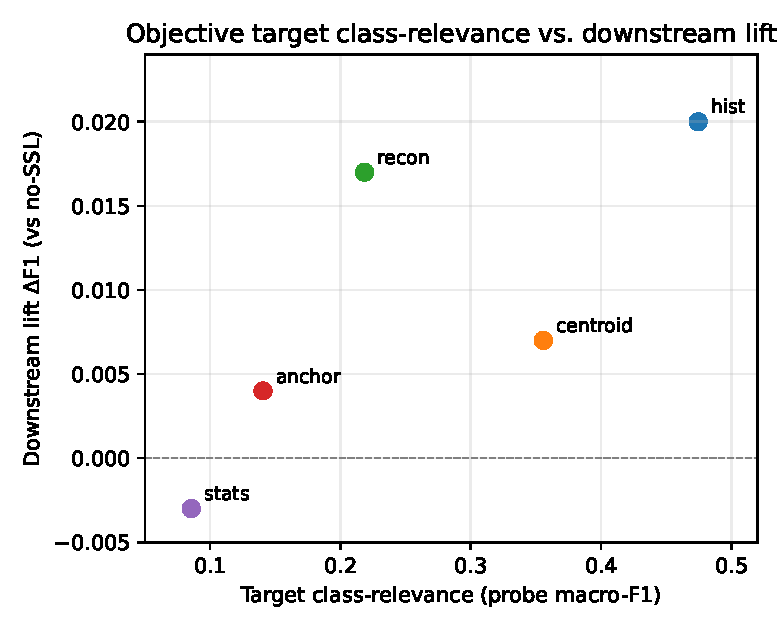
\includegraphics[width=0.5\linewidth]{figures/figA_probe_vs_lift.pdf}
% \caption{Target class-relevance versus downstream lift for per-node-target objectives. Each objective's target is probed for class information (x-axis); the more class-relevant the target, the larger the downstream improvement (y-axis). The label-histogram (hist) is highest on both; the neighbor-spread target (stats) is lowest and the only one that does not help.}
% \label{fig:probe-vs-lift}
% \end{figure}

\begin{figure}[t]
\centering
    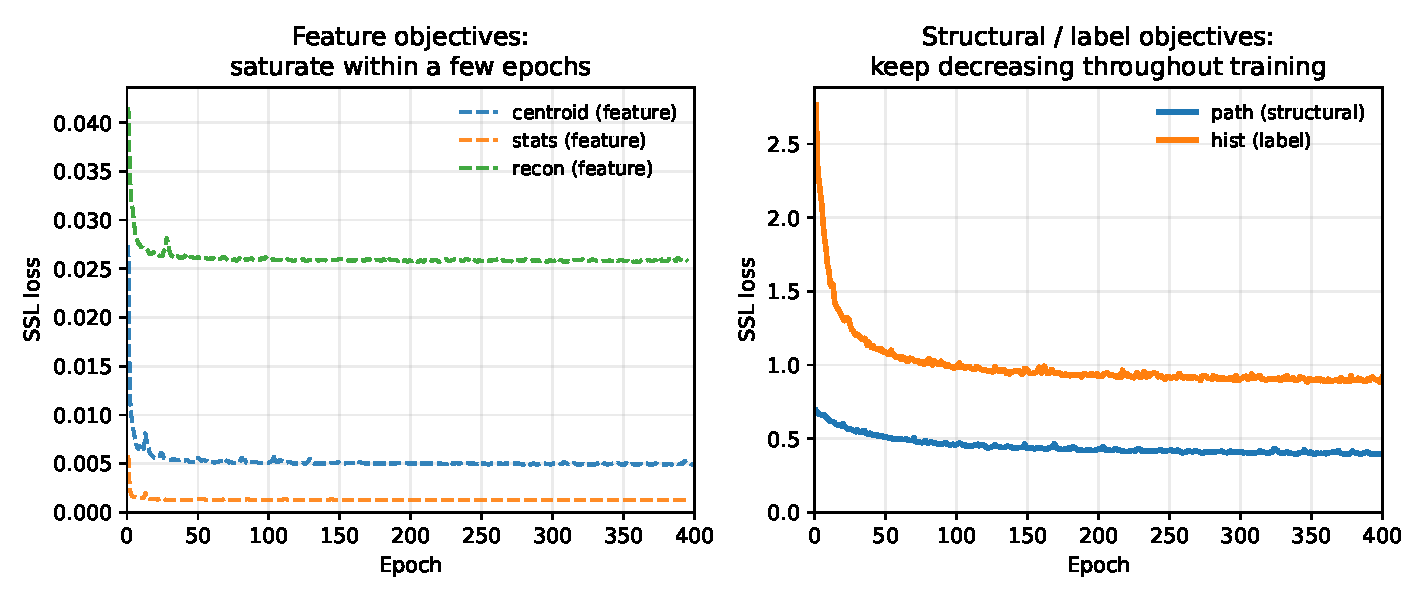
\includegraphics[width=0.8\linewidth]{figures/e10_loss_curves.pdf}
\caption{Per-objective self-supervised loss over training (each curve is from a run using that objective alone). Left: feature objectives saturate within a few epochs. Right: structural and label objectives keep decreasing throughout training.}
\label{fig:loss-curves}
\vspace{-20pt}
\end{figure}





  \begin{figure}[t]
  \centering
  \begin{minipage}[b]{0.40\linewidth}
    \centering
    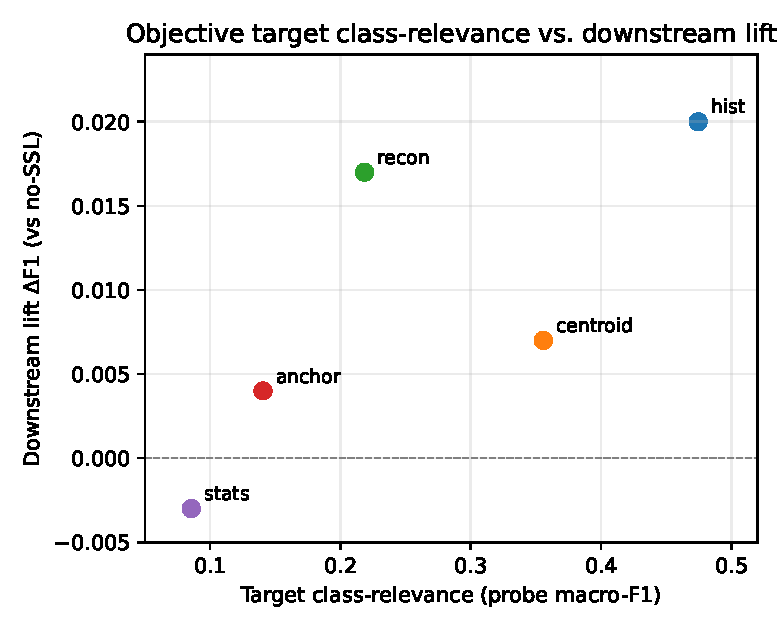
\includegraphics[width=\linewidth]{figures/figA_probe_vs_lift.pdf}
  \end{minipage}\hfill
  \begin{minipage}[b]{0.42\linewidth}
    \centering
    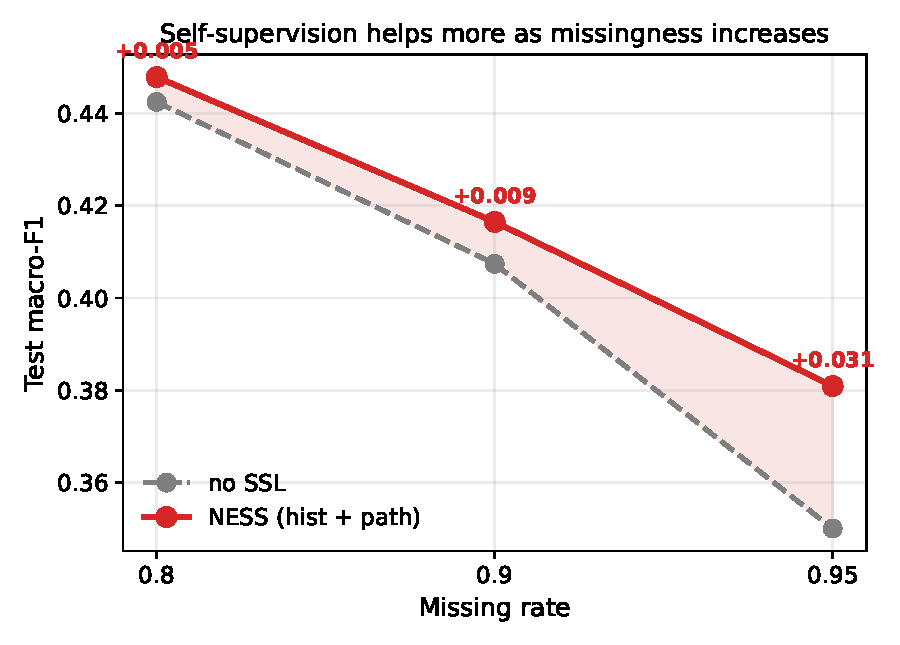
\includegraphics[width=\linewidth]{figures/e12_missingness.pdf}
  \end{minipage}

  \caption{(Left) Target class-relevance versus downstream lift for per-node-target objectives. Each objective's target is probed for class information (x-axis); the more class-relevant the target, the larger the downstream improvement (y-axis).}
  \label{fig:probe-vs-lift}
\vspace{-17pt}
  \caption{(Right) Test macro-F1 on ogbn-arxiv as the missing rate increases. Both NESS (hist + path) and the no-SSL baseline decline, but the self-supervised model declines more slowly.}
  \label{fig:missingness}
  \vspace{-20pt}
  \end{figure}



\subsection{Self-Supervision under Severe Missingness}
\label{sec:exp-missingness-regime}

The benefit of self-supervision depends on how much the encoder is starved of features. To make this precise, we compare NESS (with its hist and path objectives) against the no-SSL baseline as the missing rate increases from $0.8$ to $0.95$ on ogbn-arxiv. Figure~\ref{fig:missingness} shows the result. Both configurations degrade as features become scarcer, but the no-SSL baseline degrades faster, so the advantage of self-supervision widens: the gain over no-SSL grows from $+0.005$ at $\rho=0.8$ to $+0.031$ at $\rho=0.95$. When observed features are abundant the encoder already recovers most of the signal and self-supervision adds little; as the graph becomes information-starved, the self-supervised objectives contribute an increasingly large share of the usable signal. This is the regime in which self-supervision is most valuable.

% \begin{figure}[t]
% \centering
% 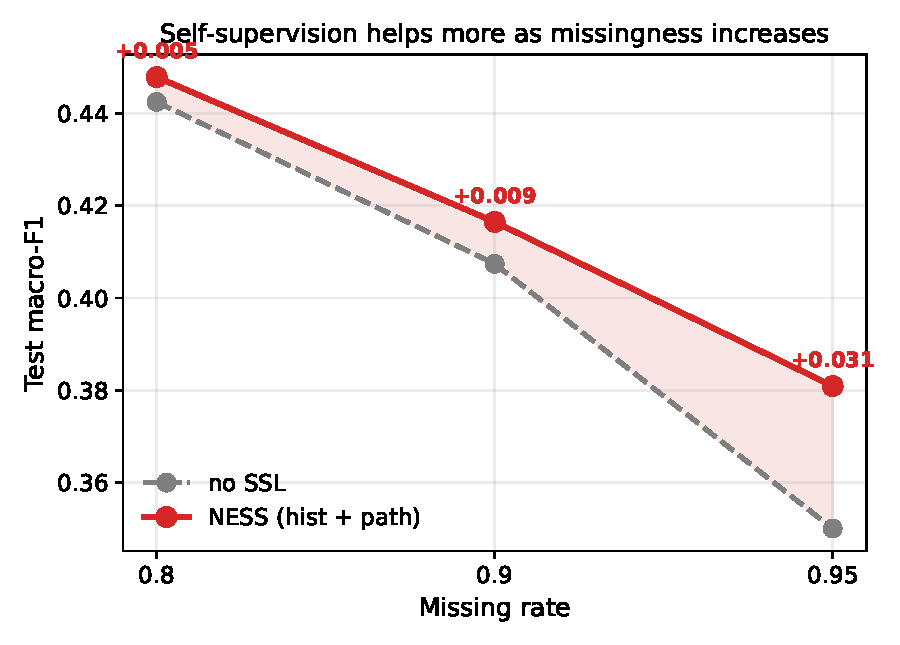
\includegraphics[width=0.6\linewidth]{figures/e12_missingness.pdf}
% \caption{Test macro-F1 on ogbn-arxiv as the missing rate increases. Both NESS (hist + path) and the no-SSL baseline decline, but the self-supervised model declines more slowly; the gap (shaded) grows from $+0.005$ at $80\%$ missing to $+0.031$ at $95\%$.}
% \label{fig:missingness}
% \end{figure}



\subsection{The Feature Regime}
\label{sec:exp-regime}

The benefit of self-supervision also depends on the type of node features. Neighborhood-centric objectives are built from aggregates of neighbor features, which are informative only when the features themselves are informative under aggregation. To test this, we apply the two label- and structure-based objectives (hist and path) to the four small graphs, whose attributes are sparse binary bag-of-words vectors, and compare the resulting lift to that observed on the dense-embedding graph ogbn-arxiv. Table~\ref{tab:regime} reports test macro-F1 at $80\%$ missingness.

On the sparse binary graphs the objectives provide essentially no benefit: the change relative to the no-SSL baseline is within $\pm 0.01$ on all four datasets, with no consistent direction. This contrasts sharply with the dense-embedding graph, where the same objectives improve macro-F1 by $0.020$. The explanation is mechanistic: neighborhood-centric targets require averaging neighbor features, which yields a meaningful, predictable signal for dense continuous attributes but is close to noise for sparse binary indicators. Neighborhood self-supervision is therefore effective in the dense-feature regime, which is both the practically prevalent one and the setting on which we focus.

\begin{table}[t]
\centering
\caption{Self-supervision on sparse binary graphs at $80\%$ missingness, with the dense-embedding result (ogbn-arxiv) for reference. On binary attributes the change over no-SSL is within noise; on dense features it is clearly positive.}
\label{tab:regime}
\small
\begin{tabular}{@{}lccc@{}}
\toprule
\textbf{Dataset} & \textbf{Features} & \textbf{no-SSL} & \textbf{$\Delta$ with SSL} \\
\midrule
Cora        & binary  & 0.798 & $0.000$ \\
CiteSeer    & binary  & 0.595 & $+0.002$ \\
AMAC        & binary  & 0.863 & $-0.005$ \\
AMAP        & binary  & 0.876 & $+0.000$ \\
\midrule
ogbn-arxiv  & dense   & 0.424 & $+0.020$ \\
\bottomrule
\end{tabular}
\end{table}


\subsection{Design Choices and Sensitivity}
\label{sec:exp-design}

We now justify NESS's design choices and show that its performance is not brittle to hyperparameters. All studies are on ogbn-arxiv at $80\%$ missingness.

\paragraph{Design choices:} Figure~\ref{fig:design} compares the two principal architectural decisions, each varied in isolation. For the encoder, GraphSAGE outperforms GAT and GCN; its separate self-transformation preserves each node's prefilled signal through depth, unlike GCN-style aggregation that mixes a node's own signal with its neighbors' in a single term. For the prefill, Feature Propagation clearly outperforms a single round of neighbor-mean imputation and zero-filling, confirming that long-range diffusion recovers signal that a single aggregation step or no imputation cannot. (The two panels are separate ablations and share only the metric axis; absolute values are not directly comparable across them.)

\paragraph{Component ablation:} Table~\ref{tab:components} removes NESS's learning components one at a time. Removing the self-supervised objectives (no-SSL) and, more so, the entire two-view contrastive structure (single-view) both reduce performance, and removing the Feature-Propagation prefill (zero-fill) is the most damaging. Each component contributes, and the prefill is the single most important.

\paragraph{Hyperparameter sensitivity:} Figure~\ref{fig:hp} varies four hyperparameters one at a time around the chosen configuration; all values are selected on validation performance. Performance is stable, and the chosen settings lie within a stable region: a deeper (three-layer) encoder and lower dropout ($0.3$) are preferable, and the learning rate is stable around $10^{-3}$. Up-weighting the classification term improves results and then plateaus; we set its weight to $3$, a stable point on this plateau rather than the extreme, to avoid over-emphasizing the supervised term at the expense of the auxiliary signal that matters at higher missingness.

\begin{figure}[t]
\centering
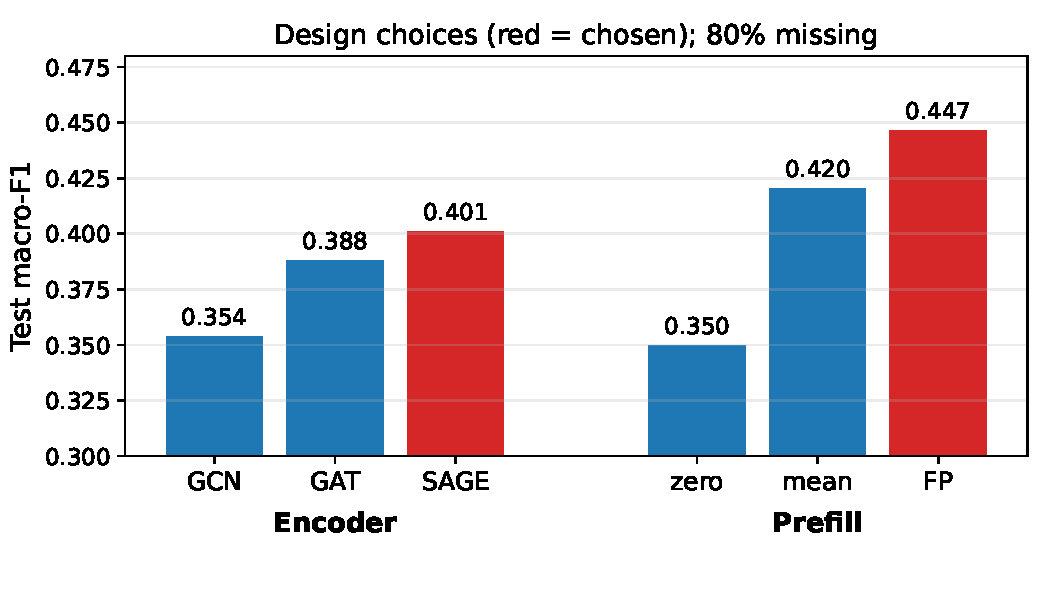
\includegraphics[width=0.7\linewidth]{figures/e11_design_choices.pdf}
\vspace{-20pt}
\caption{Design choices (chosen option in red), on ogbn-arxiv at $80\%$ missingness. GraphSAGE is the best encoder and Feature Propagation the best prefill. The two panels are independent ablations.}
\label{fig:design}
\vspace{-20pt}
\end{figure}

\begin{figure}[t]
\centering
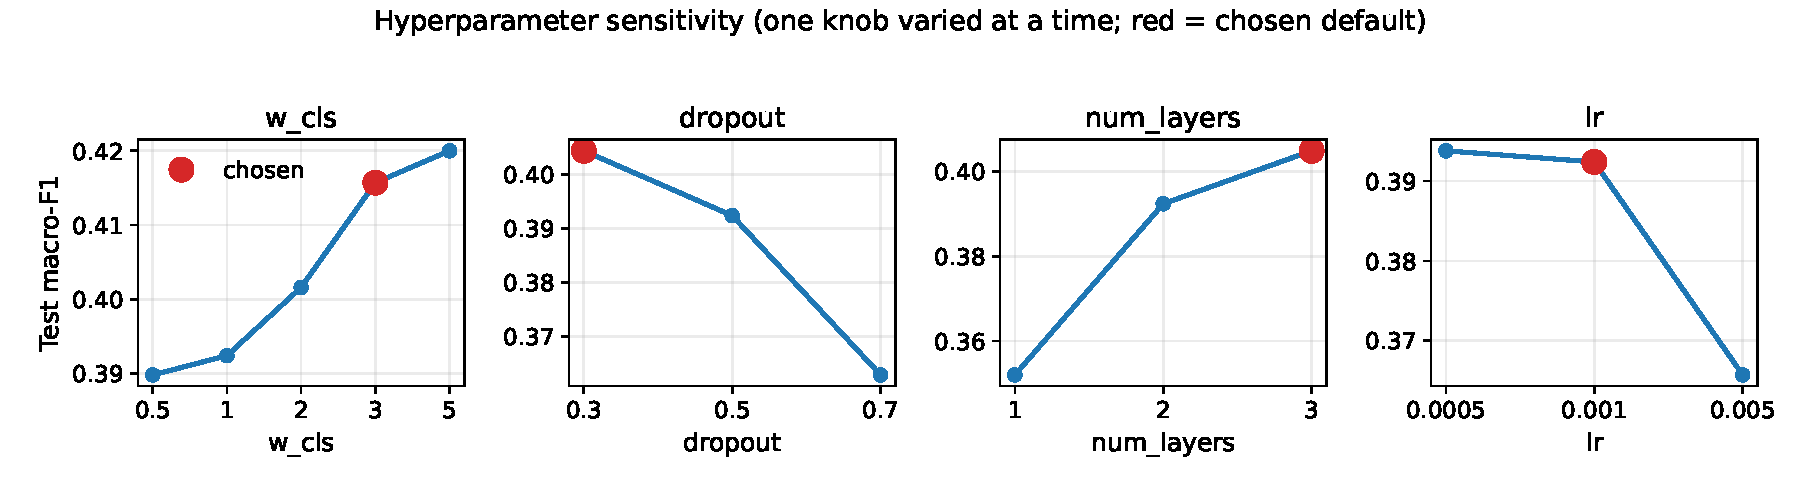
\includegraphics[width=\linewidth]{figures/e11_hp_sensitivity.pdf}
\caption{Hyperparameter sensitivity: each knob is varied with the others fixed; the chosen default is marked in red. Performance is stable, and the selected settings lie within a stable region.}
\label{fig:hp}
\end{figure}


\begin{table}[t]
\centering
\vspace{-25pt}
\caption{Component ablation on ogbn-arxiv at $80\%$ missingness (test macro-F1, three seeds). Removing any learning component reduces performance; the prefill matters most.}
\label{tab:components}
\small
\begin{tabular}{@{}lc@{}}
\toprule
\textbf{Configuration} & \textbf{Test F1} \\
\midrule
NESS (full)                       & \textbf{0.447} \\
\;\; without SSL objectives       & 0.424 \\
\;\; without two-view contrastive & 0.416 \\
\;\; without FP prefill (zero-fill) & 0.350 \\
\bottomrule
\end{tabular}
\end{table}




\subsection{Transferability of the Objective}
\label{sec:exp-transfer}

To show that an effective SSL objective reflects a general principle rather than a property of our architecture, we test whether it improves other backbones as well. We add the label-histogram objective to two baselines, GraphSAGE and PaGCN, as an auxiliary loss and measure the change in test macro-F1 on ogbn-arxiv at $80\%$ missingness. Table~\ref{tab:transfer} shows that both backbones improve when the objective is added, indicating that the benefit transfers across architectures and is driven by the objective rather than by NESS specifically. The gains are modest, consistent with the objective supplying a semi-supervised signal that is most valuable where the backbone is otherwise weak.

\begin{table}[t]
\centering
\caption{Adding the label-histogram objective to other backbones (on ogbn-arxiv, $80\%$ missingness, macro-F1).}
\label{tab:transfer}
\small
\begin{tabular}{@{}lccc@{}}
\toprule
\textbf{Backbone} & \textbf{without} & \textbf{with hist} & \textbf{$\Delta$} \\
\midrule
GraphSAGE & 0.217 & 0.229 & $+0.012$ \\
PaGCN     & 0.300 & 0.318 & $+0.018$ \\
\bottomrule
\end{tabular}
\end{table}




\subsection{Scalability}
\label{sec:exp-scalability}

Finally, we confirm that NESS is practical at scale. Figure~\ref{fig:scalability} plots test macro-F1 against peak GPU memory for all methods on ogbn-arxiv, with bubble size indicating training time. NESS attains the highest macro-F1 at a peak memory of $1.3$~GB, comparable to the per-node baseline (MATE) and well within a single GPU; its self-supervised objectives and prefill add only a small memory overhead relative to a standard clustered GNN. Its training time is higher than the simpler baselines (larger bubble), reflecting the auxiliary objectives computed each epoch, but remains on the order of minutes on a single GPU.

\begin{figure}[t]
\centering
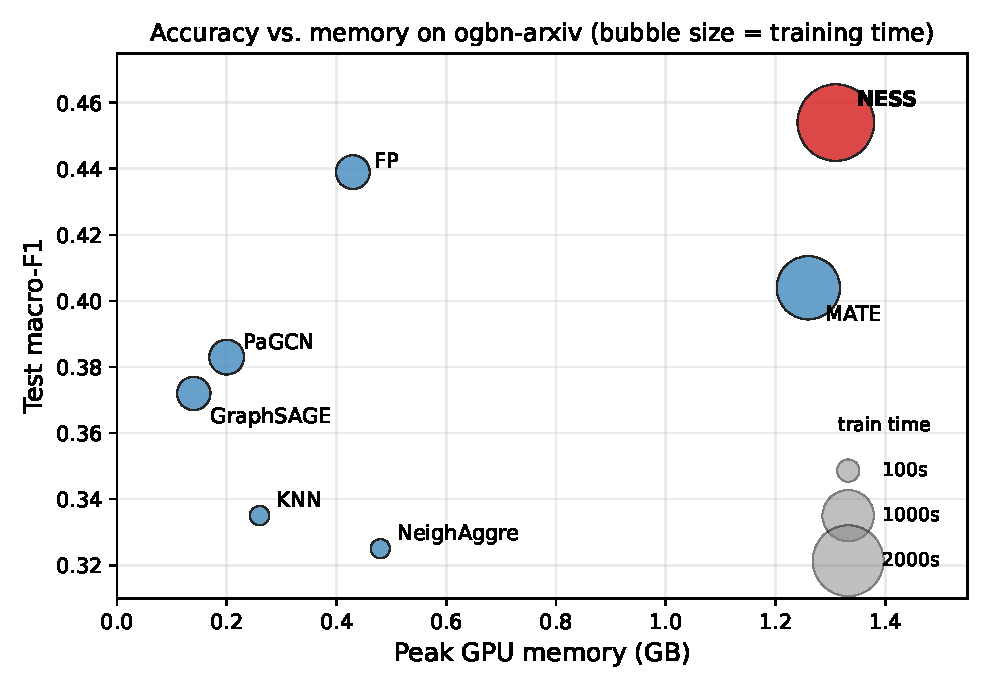
\includegraphics[width=0.6\linewidth]{figures/e6_scalability_bubble.pdf}
\caption{Macro-F1 versus peak GPU memory on ogbn-arxiv at $80\%$ missingness; bubble size is training time. NESS (red) attains the highest macro-F1 at memory comparable to other GNNs, confirming it scales with manageable memory usage.}
\label{fig:scalability}
 \vspace{-20pt} 

\end{figure}
% \vspace{-6pt} 


